In diesem abschließenden Kapitel möchten wir nun die in
\Cref{chap:implementation} beschriebene Realisierung von
\Cref{alg:primalDualIteration} mit Abbruchkriterium
\eqref{eq:terminationCriterion} im Solve-Schritt der AFEM-Schleife aus
\Cref{fig:afemLoop} an einigen Benchmark-Problemen untersuchen.
Dabei benutzen wir die Bezeichnungen aus \Cref{alg:primalDualIteration}.
Zunächst möchten wir alle Parameterwahlen aufführen, die in allen 
Experimenten gleich gesetzt werden, sofern nicht anders angegeben.
Als Startwert für die Iteration auf dem ersten Level wählen wir
$u_0\equiv 0$ und auf den darauffolgenden Leveln eine Prolongation wie zum
Ende von \Cref{sec:programFlow} beschrieben.
Für jeden Aufruf der primalen-dualen Iteration wählen wir $\Lambda_0$ wie in
\Cref{eq:choiceInitialDualVariableImplementation} angegeben.
Dabei konstruieren wir Probleme, bei denen die exakte Lösung bekannt ist,
nach \Cref{sec:constructionInputSignal}. 
Bei diesen ist ein Argument $r$ stets aus $[0,\infty)$.
Als besonderes Augenemerk betrachten wir dabei zwei Eingangssignale.
Andere Funktionen werden wir bei Bedarf betrachten, um bestimmte Eigenschaften
zu untersuchen im Vergleich zu diesen beiden Benchmark-Problemen.
Für ein Experiment mit exakter Lösung betrachten wir für einen Parameter
$\beta\geq 1/2$, wobei wir $\beta =1$ wählen, die Funktion
\begin{align*}
  u(r)&\coloneqq
  \begin{cases}
    1, 
    & \text{falls } r\in \left[0,\frac{1}{6}\right],\\
    1+(6r-1)^\beta, 
    & \text{falls } r\in \left(\frac{1}{6}, \frac{1}{3}\right],\\
    2, 
    & \text{falls } r\in \left(\frac{1}{3}, \frac{1}{2}\right],\\
    2\left(\frac{5}{2}-3r\right)^\beta, 
    & \text{falls } r\in \left(\frac{1}{2}, \frac{5}{6}\right],\\
    0, 
    & \text{falls } r\in \left(\frac{5}{6}, \infty\right),\\
  \end{cases}
\end{align*}
und wählen
\begin{align*}
  \sgn\big(\partial_r u(r)\big) 
  &\coloneqq
  \begin{cases}
    12r-36r^2, 
    & \text{falls } r\in \left[0,\frac{1}{6}\right],\\
    1, 
    & \text{falls } r\in \left(\frac{1}{6}, \frac{1}{3}\right],\\
    \cos(\pi(6r-2)), 
    & \text{falls } r\in \left(\frac{1}{3}, \frac{1}{2}\right],\\
    -1, 
    & \text{falls } r\in \left(\frac{1}{2}, \frac{5}{6}\right],\\
    -\frac{1+\cos(\pi(6r-5))}{2}, 
    & \text{falls } r\in \left(\frac{5}{6}, \infty\right).
  \end{cases}
\end{align*}
Nach \Cref{eq:constructionInputSignal} ist $u$ mit dieser Wahl von
$\sgn\big(\partial_r u\big)$ die Lösung von \Cref{prob:continuousProblem} mit
Eingangssignal
\begin{align*}
  f(r)
  &=
  \begin{cases}
    \alpha-12(2-9r), 
    & \text{falls } r\in \left[0,\frac{1}{6}\right],\\
    \alpha\left(1+(6r-1)^\beta\right)-\frac{1}{r}, 
    & \text{falls } r\in \left(\frac{1}{6}, \frac{1}{3}\right],\\
    2\alpha+6\pi\sin(\pi(6r-2))-\frac{1}{r}\cos(\pi(6r-2)), 
    & \text{falls } r\in \left(\frac{1}{3}, \frac{1}{2}\right],\\
    2\alpha\left(\frac{5}{2}-3r\right)^\beta+\frac{1}{r},
    & \text{falls } r\in \left(\frac{1}{2}, \frac{5}{6}\right],\\
    -3\pi\sin(\pi(6r-5))+\frac{1+\cos(\pi(6r-5))}{2r}, 
    & \text{falls } r\in \left(\frac{5}{6}, \infty\right).
  \end{cases}
\end{align*}
Ebenfalls nach \Cref{sec:constructionInputSignal} können die schwachen
Gradienten von $u$ und $f$ bestimmt werden mithilfe der partiellen 
Ableitungen

\begin{align*}
  \partial_r f(r)
  &=
  \begin{cases}
    108,
    & \text{falls } r\in\left[0,\frac{1}{6}\right],\\
    6\alpha\beta(6r-1)^{\beta-1} +\frac{1}{r^2}, 
    & \text{falls } r\in\left(\frac{1}{6},\frac{1}{3}\right],\\
    \left(36\pi^2+\frac{1}{r^2}\right)\cos(\pi(6r-2))
    + \frac{6\pi}{r}\sin(\pi(6r-2)), 
    & \text{falls } r\in\left(\frac{1}{3},\frac{1}{2}\right],\\
    -\left(6\alpha\beta\left( \frac{5}{2}-3r \right)^{\beta-1}+
    \frac{1}{r^2}\right),
    & \text{falls } r\in\left(\frac{1}{2},\frac{5}{6}\right],\\
    -\left( \left( 18\pi^2+\frac{1}{2r^2} \right)\cos(\pi(6r-5))
    +\frac{1}{2r^2} + \frac{3\pi}{r}\sin(\pi(6r-5))\right), 
    &\text{falls } r\in\left(\frac{5}{6},\infty\right),
  \end{cases}
\end{align*}
und 
\begin{align*}
  \partial_r u(r) 
  &= 
  \begin{cases}
    0,
    & \text{falls } r\in\left[0,\frac{1}{6}\right],\\
    6\beta(6r-1)^{\beta-1}, 
    & \text{falls } r\in\left(\frac{1}{6},\frac{1}{3}\right],\\
    0, 
    & \text{falls } r\in\left(\frac{1}{3},\frac{1}{2}\right],\\
    -6\beta\left( \frac{5}{2}-3r \right)^{\beta-1},
    & \text{falls } r\in\left(\frac{1}{2},\frac{5}{6}\right],\\
    0,
    &\text{falls } r\in\left(\frac{5}{6},\infty\right).
  \end{cases}
\end{align*}
Durch Kenntnis des schwachen Gradienten von $u$ erhalten wir für die
exakte Energie die Approximation $E(u)\approx -2.05803442842497$, mit der
wir die Ergebnisse der Experimente vergleichen können.
\begin{figure}[!ht]
  \centering
  \begin{subfigure}[b]{.48\linewidth}
    \caption{$f$}
    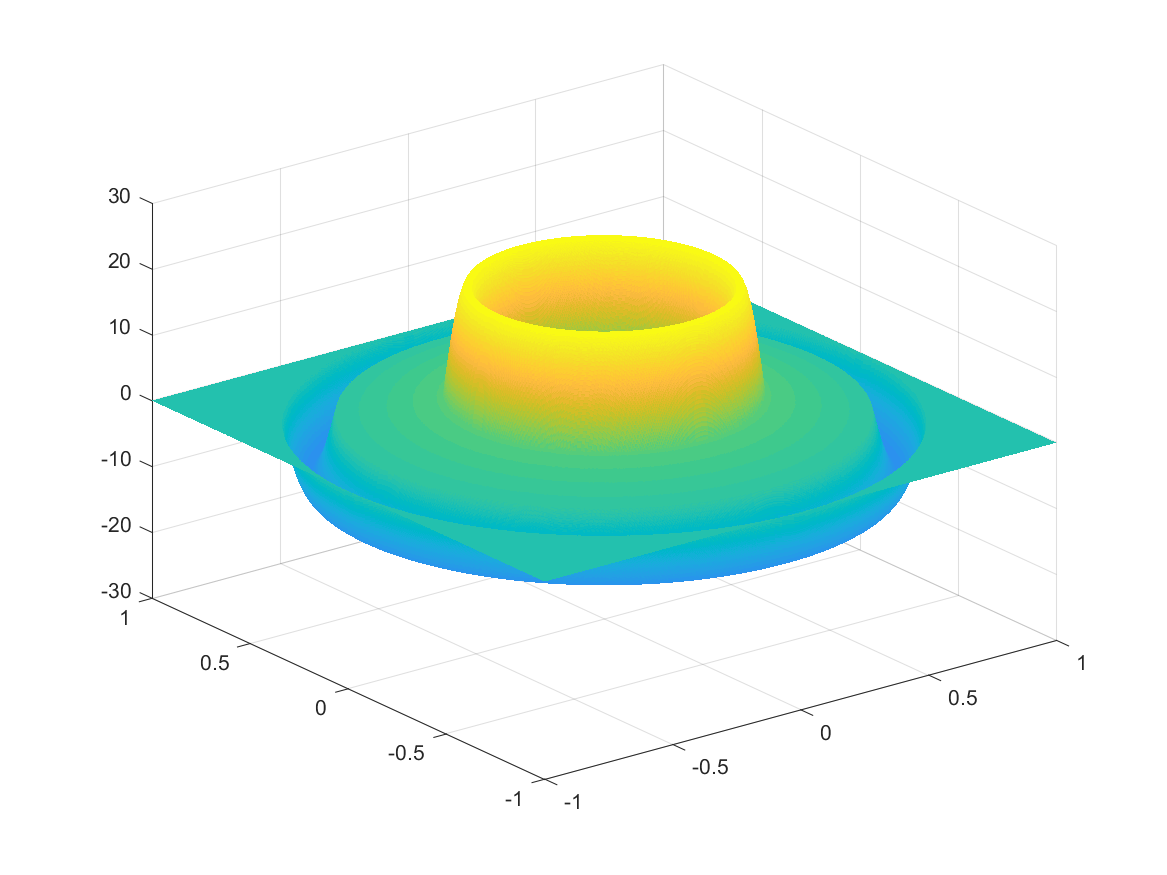
\includegraphics[trim = 40 30 30 30, clip, width=\linewidth]
      {pictures/chapExperiments/secGeneralInfo/f01Plots/inSi.png}
    \label{fig:f01InSi}
  \end{subfigure}
  \quad
  \begin{subfigure}[b]{.48\linewidth}
    \caption{$u$}
    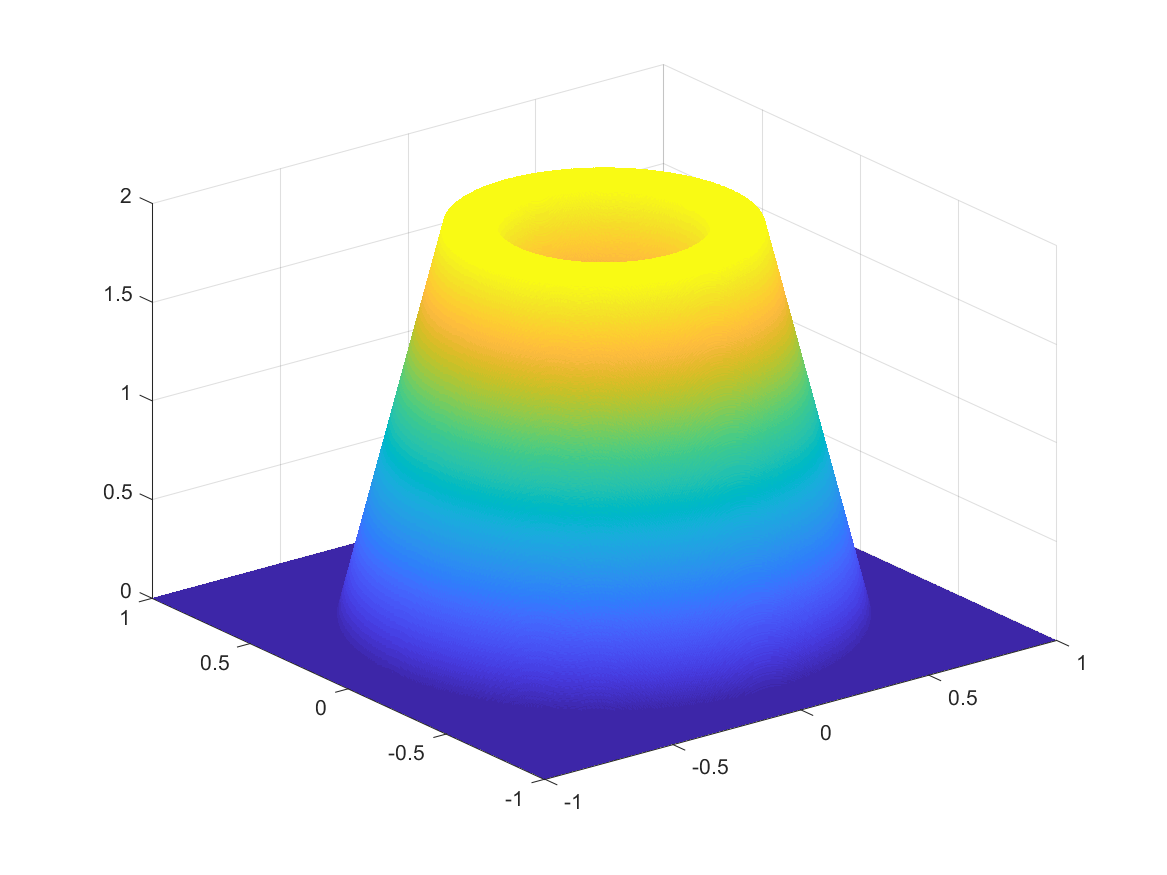
\includegraphics[trim = 40 30 30 30, clip, width=\linewidth]
      {pictures/chapExperiments/secGeneralInfo/f01Plots/exactSolution.png}
    \label{fig:f01ExactSol}
  \end{subfigure}

  \begin{subfigure}[b]{.48\linewidth}
    \caption{$f$ entlang der x- und y-Achse}
    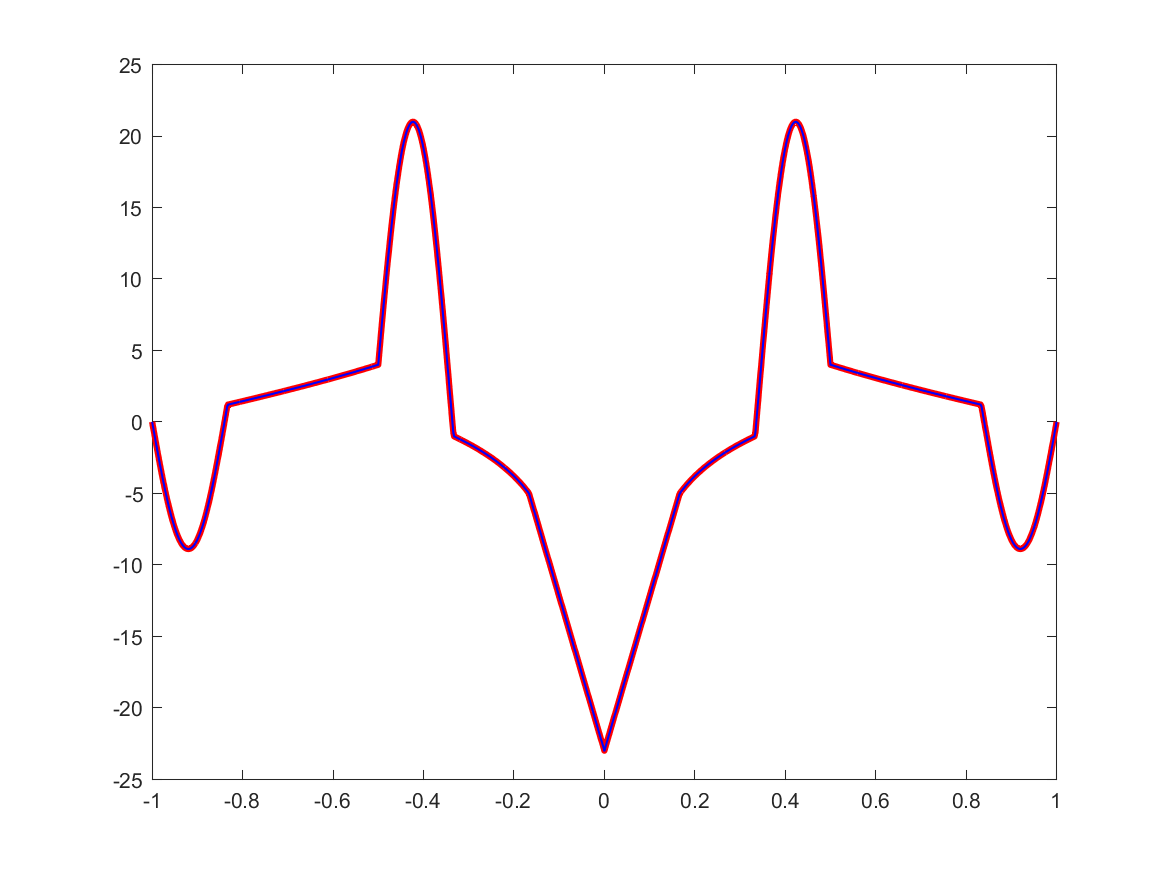
\includegraphics[trim = 50 30 50 20, clip, width=\linewidth]
      {pictures/chapExperiments/secGeneralInfo/f01Plots/inSiAxis.png}
    \label{fig:f01InSiAxis}
  \end{subfigure}
  \quad
  \begin{subfigure}[b]{.48\linewidth}
    \caption{$u$ entlang der x- und y-Achse}
    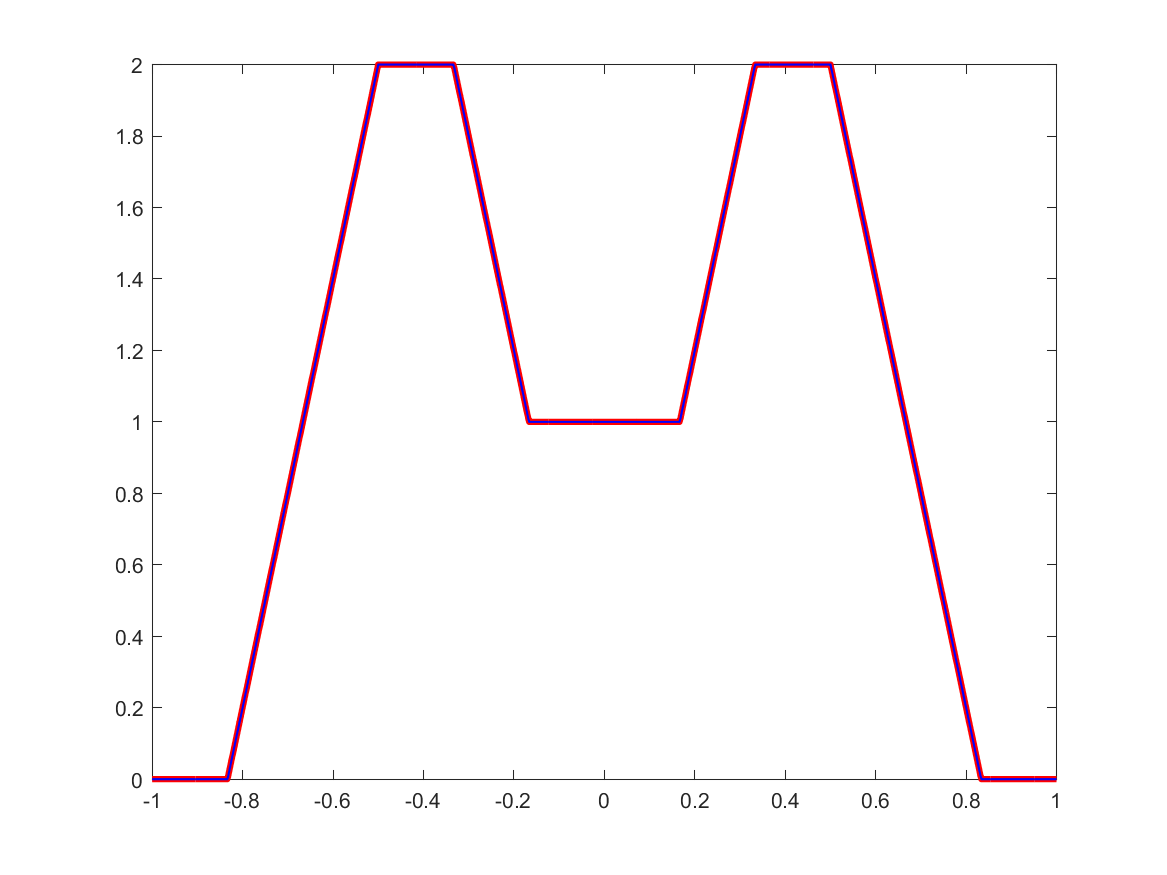
\includegraphics[trim = 50 30 50 20, clip, width=\linewidth]
      {pictures/chapExperiments/secGeneralInfo/f01Plots/exactSolutionAxis.png}
    \label{fig:f01ExactSolAxis}
  \end{subfigure} 
  \caption{Eingangssignal $f$ und exakte Lösung $u$ sowie deren
  Darstellungen entlang der x-Achse (blau) und der y-Achse (rot) für
  $\alpha=1$.}
  \label{fig:f01Plots}
\end{figure}
Als initiale Geometrie, das heißt die Geometrie für das erste Level des
AFEM-Algorithmus, nutzen wir in den Experimenten mit exakter Lösung
\texttt{BigSquare} des AFEM-Pakets ohne initiale Rotverfeinerung, zu sehen in
\Cref{fig:triangBigSquare}, da diese den Einheitskreis, das heißt den Träger
des Eingangssignals und der exakten Lösung nach
\Cref{sec:constructionInputSignal}, enthält.
Wenn nicht anders angegeben, dann betrachten wir dieses Beispiel stets mit
$\alpha=1$.

Für ein Problem mit unstetigem Eingangssignal legen wir besonderes
Augenmerk auf das Graufarbenbild \texttt{cameraman} aus \cref{fig:cameraman}
als Eingangssignal. 
Wenn nicht anders angegeben, dann betrachten wir dieses Beispiel stets mit
$\alpha=10^4$.
Auch für dieses komplexere Beispiel, bei der selbst eine stückweise
Beschreibung durch Polynome augenscheinlich nur schwer möglich ist, sowie in
allen weiteren Experimenten haben selbst deutlich höhere Integrationsgrade als
$10$ zu keinen veränderten Raten geführt. 
Diese Wahl des Integrationsgrads erscheint daher als ausreichend.
Da außerdem in dieser Implementierung darauf geachtet wurde, die
\texttt{integrate} Methode des AFEM-Softwarepakets \cite{Car09} nicht während
der primalen-dualen Iteration aufzurufen, hat eine möglicherweise zu hohe Wahl
des Integrationsgrads keinen relevanten Effekt auf die Programmlaufzeit und
kann somit ohne Sorge als 10 gewählt werden.
Diese Wahl des Integrationsgrads gilt nur für die Methode \texttt{errorCRL2}
des AFEM-Softwarepakets zur Berechnung des Fehlers nicht, da diese unverändert
übernommen wurde und den Grad 12 nutzt.
Fur Experiment mit Graufarbenbild als Eingangssignal nutzen wir als initiale
Triangulierung \texttt{Square} des AFEM-Softwarepakets ohne initiale
Rotverfeinerung, zu sehen in \Cref{fig:triangSquare}.

\begin{figure}[!ht]
  \centering
  \begin{subfigure}[b]{.48\linewidth}
    \caption{\texttt{BigSquare}}
    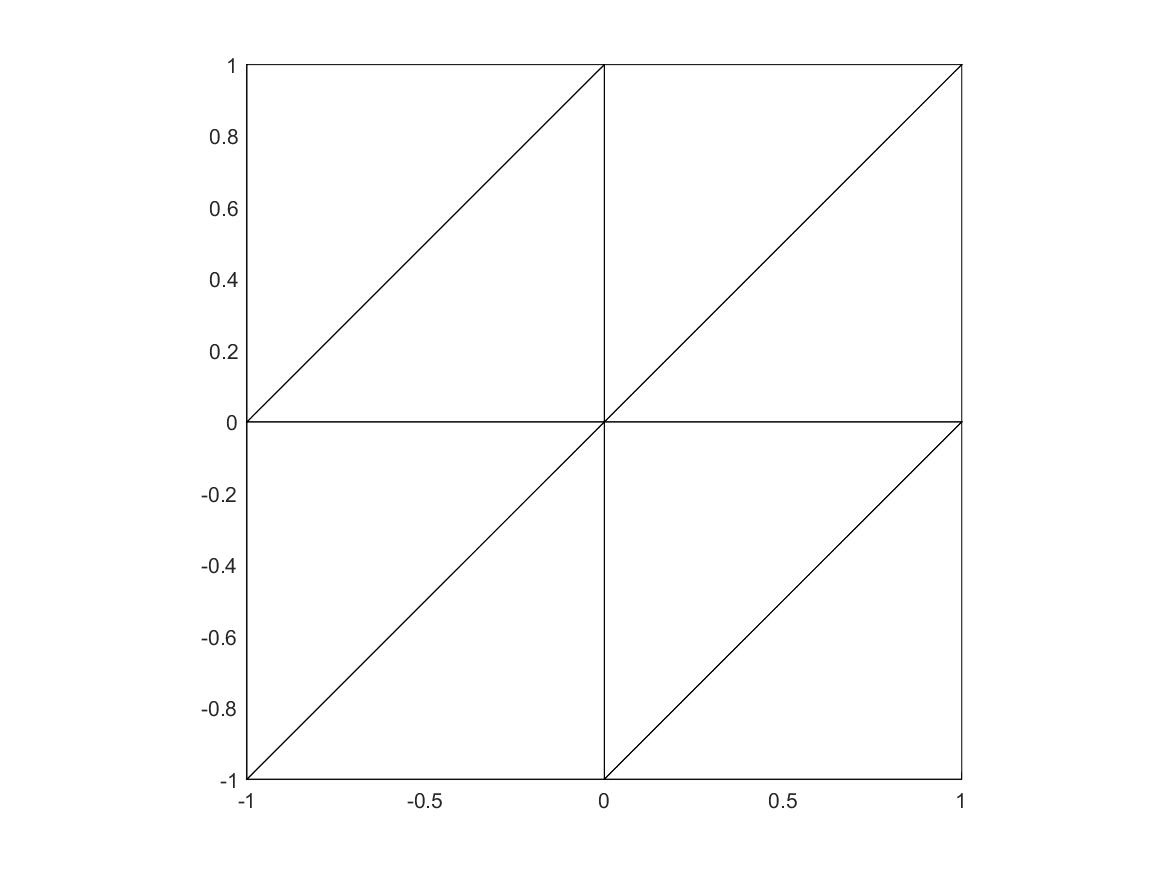
\includegraphics[trim = 90 30 90 20, clip, width=\linewidth]
      {pictures/chapExperiments/secGeneralInfo/bigSquareTriang.png}
    \label{fig:triangBigSquare}
  \end{subfigure}
  \quad
  \begin{subfigure}[b]{.48\linewidth}
    \caption{\texttt{Square}}
    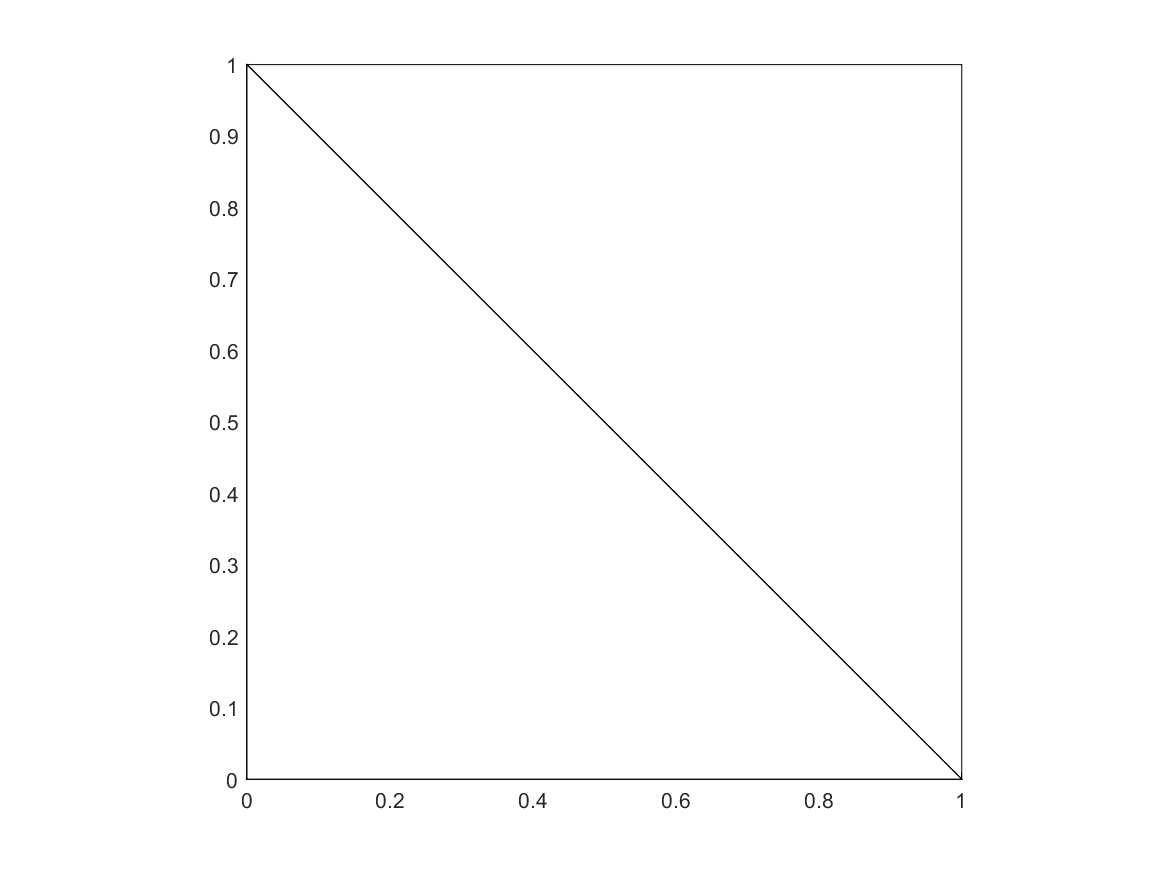
\includegraphics[trim = 90 30 90 20, clip, width=\linewidth]
      {pictures/chapExperiments/secGeneralInfo/squareTriang.png}
    \label{fig:triangSquare}
  \end{subfigure}
  \caption{In den Experimenten genutzte initiale Triangulierung.}
  \label{fig:initialTriangulations}
\end{figure}
Führen wir ein Experiment mit adaptiver Netzverfeinerung durch, so wählen wir
den Bulk-Parameter für den Mark-Schritt des AFEM-Algorithmus $\theta=0.5$.
Auf die Wahl der Parameter $\tau$ und $\epsstop$ für die primale-duale
Iteration werden wir im folgenden \Cref{sec:choiceOfParameters} eingehen.
Zur Wahl des Parameters $\gamma$ auf dem Verfeinerungsindikator betrachten
wir in \Cref{sec:experimentsWithExactSolution} ein Beispiel.
Die maximale Iterationszahl ist, mit Ausnahme von einem Experimente in
\Cref{sec:choiceOfParameters}, smit $10^{12}$ so gewählt, dass diese nie 
der Grund für das Beenden einer primalen-dualen Iteration ist, also stets das
Abbruchkriterium aus \eqref{eq:terminationCriterion} für den Abbruch
verantwortlich ist.
Die minimale Anzahl der Freiheitsgrade ist so gewählt, dass AFEM-Routine
manuell oder durch Server beendet wird, bevor Sie durch erreichen 
der Freiheitsgrade beendet wird. Dies geschah in allen Experimenten bei 
etwa $10^6$ Freiheitsgraden.


\section{Wahl der Parameter für die primale-duale Iteration}
\label{sec:choiceOfParameters}

Zunächst interessiert und die Wahl des Parameters $\tau$ in 
\Cref{alg:primalDualIteration}. 
Diesen müssen wir nach \Cref{thm:convergenceIteration} in $(0,1]$ wählen um
Konvergenz der primalen-dualen Iteration zu garantieren.
Der Parameter $\epsstop$ wird mit $10^{-4}$ gewählt. Diese Wahl wird 
anschließend ebenfalls nochmal näher betrachtet. Außerdem wird $\theta=0.5$
gewählt. Außerdem werden (ggf hier noch weitere nicht-standart params nennen 
und deren Wahl).

\begin{figure}[!ht]
  \centering
  \begin{subfigure}[b]{.48\linewidth}
    \caption{Eingangssignal $f$}
    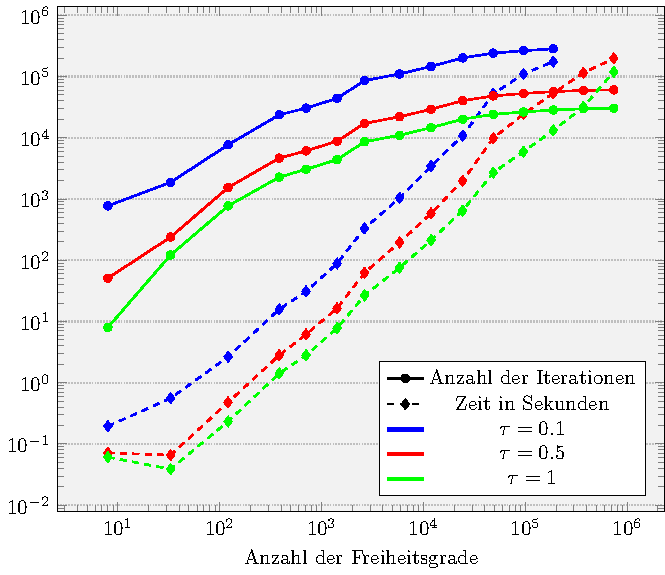
\includegraphics[width=\linewidth]
      {pictures/chapExperiments/secParameters/parTau/f01/miscF.pdf}
    \label{fig:parTauMiscF}
  \end{subfigure}
  \quad
  \begin{subfigure}[b]{.48\linewidth}
    \caption{Eingangssignal \texttt{cameraman}}
    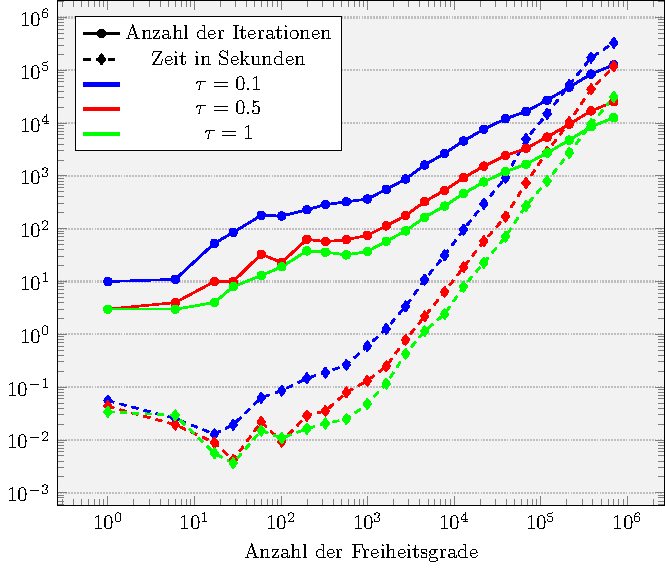
\includegraphics[width=\linewidth]
      {pictures/chapExperiments/secParameters/parTau/cam/miscCam.pdf}
    \label{fig:parTauMiscCam}
  \end{subfigure}
  \caption{Anzahl der Iterationen und benötigte Zeit für verschiedene Werte
  von $\tau$ mit den Eingangssignalen $f$ und \texttt{cameraman}.}
  \label{fig:parTauMisc}
\end{figure}

\begin{figure}[!ht]
  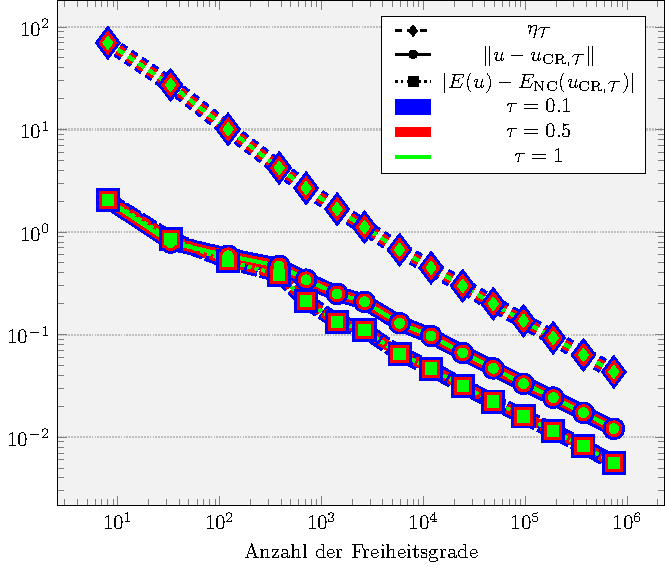
\includegraphics[width=\linewidth]
    {pictures/chapExperiments/secParameters/parTau/f01/convergenceF.pdf}
  \caption{Verfeinerungsindikator, exakter $L^2$-Fehler und Energiedifferenz 
  für verschieden Werte von $\tau$ mit Eingangangssignal $f$.}
  \label{fig:parTauConvergence}
\end{figure}

Wie in \Cref{fig:parTauMisc} zu sehen, verhält sich die Anzahl der Iteration,
und damit, wie zu erwarten war, auch die Laufzeit, antiproportional zur Größe
der hier gewählten Werte von $\tau$.
Da sich die betrachteten Graphen in \Cref{fig:parTauConvergence} für die
verschiedenen Wahlen von $\tau$ nicht sichtbar unterscheiden, schlussfolgern
wir, dass die ideale Wahl für $\tau$, die \Cref{thm:convergenceIteration}
zulässt, das heißt $\tau=1$, zu sein scheint, da die primale-duale Iteration
bei gleichen Ergebnissen für dieses $\tau$ die geringste Laufzeit hat.
Ein mögliche Erklärung liefert der Beweis von \Cref{thm:convergenceIteration}.
Die darin bewiesene \Cref{eq:upperBoundIterationError} impliziert für die
Iterate $(u_j)_{j\in\Nbb}$, dass
\begin{align*}
  \sum_{j=1}^\infty\Vert \ucr - u_j \Vert^2 
  \leq
  \frac{1}{2\alpha\tau}
  \left(\vvvert \ucr - u_0\vvvert^2_\nc 
  + \left\Vert \bar\Lambda_0 - \Lambda_0\right\Vert^2\right). 
\end{align*}
Die rechte Seite ist antiproportional zu $\tau>0$, womit womöglich
die Folge $(\left\Vert \ucr - u_j\right\Vert)_{j\in\Nbb}$ schneller gegen $0$
konvergiert und damit auch das Abbruchkriterium \eqref{eq:terminationCriterion}
nach einer geringeren Anzahl von Iterationen erfüllt ist. 
Der Beweis von \Cref{thm:convergenceIteration} liefert uns keine
Informationen darüber, ob möglicherweise auch eine Wahl $\tau>1$ immer noch die
Konvergenz der primalen-dualen Iteration garantiert.
Wie aber in Abb \ldots zu sehen, wurde schon für $\tau=1.2$ ein Beispiel 
gefunden, bei dem nicht davon ausgegangen werden kann, dass die primale-duale
Iteration konvergiert.
Diese Iteration wurde auf der Triangulierung Abb (mglw auf Square verweisen,
da es genau die sein könnte. 
Dabei wurde die Iteration nach $10^6$ Iterationen abgebrochen, da kein anderes
Verhalten mehr zu erwarten war, zumal selbst für die nach
\Cref{fig:parTauMiscF} suboptimale Wahl $0.1$ für $\tau$ weniger also $10^3$
Iterationen auf der gleichen Triangulierung benötigt wurden und für die Wahl
$\tau=1$ sogar weniger als $10$ Iterationen.
% includegraphics tau keine Konvergenz

Nun betrachen wir die Wahl des Parameteres $\epsstop$ für das Abbruchkriterium.
Wieder wählen wir $\theta = 0.5$ und \ldots.

\begin{figure}[!ht]
  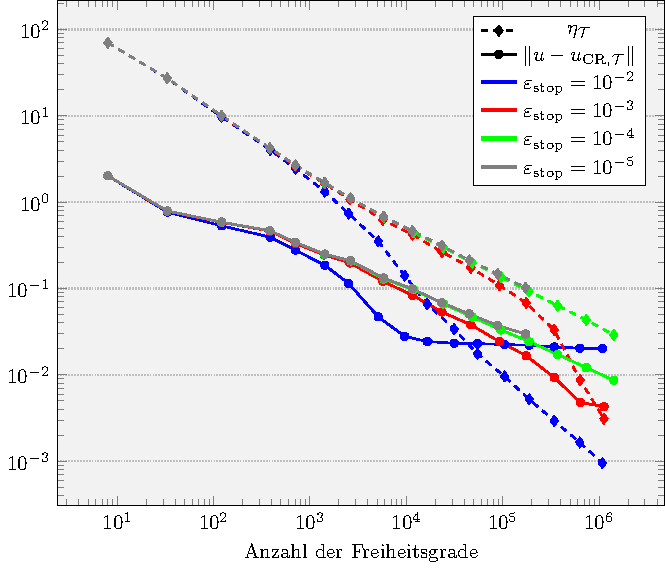
\includegraphics[width=\linewidth]
    {pictures/chapExperiments/secParameters/parEpsStop/f01/convergenceF.pdf}
  \caption{Verfeinerungsindikator und exakter $L^2$-Fehler für verschieden
  Werte von $\epsstop$ mit Eingangangssignal $f$.}
  \label{fig:parEpsStopConvergence}
\end{figure}
Wie in \Cref{fig:parEpsStopConvergence} zu sehen, stagniert der 
exakte $L^2-Fehler$ für $\epsstop=10^{-2}$ und, es lässt sich erahnen, dass
dieser Effekt auch für $\epsstop=10^{-3}$ einsetzt. 
Da der Effekt bis $10^6$ Freiheitsgrade für $\epsstop\in\{10^{-4},10^{-5}\}$
noch nicht einsetzt, scheint dies an einem zu frühen Abbruch der Iteration 
durch eine zu große Toleranz $\epsstop$ zu liegen. 
Bei hohen Freiheitsgraden und einer entsprechend kleinen Netzweite muss
also $\epsstop$ ausreichend klein gewählt werden.
Da wir in den Experimenten  $10^6$ Freiheitsgrade nicht überschreiten und
sich bis dahin die Ergebnisse für die Wahlen $10^{-4}$ und $10^{-5}$ kaum
unterscheiden bei längerer Laufzeit für $10^{-5}$, wählen wir als Standard
$\epsstop=10^{-4}$.
Weiterhin bleibt festzuhalten, dass der Verfeinerungsindikator trotzdem noch
passend Dreiecke auswählt und weiter fällt, auch bei stagnierendem Fehler.

==================


zu gamma (0, 0.5, 1) noch irgendwo ein Experiment mit Info, dass 0 und 1e-4 oder
so was identisch sind

  - gamma = 0 im Vergleich der gammas mit erwähnen (da es sich von gamma 1e-4
    nicht unterscheider visuell (nochmal prüfen ob das stimmt) nur eines der
    beiden gammas plotten und genau diese Info in einem Satz erwähnen und vlt
    auch in der Legende beides für einen Graphen angeben gamma = 0, 1e-4)

In der Abbildung ist tatsächlich $\gamma= 10^{-4}$ nicht abgebildet, da
die entsprechend Graphen sich nicht sichtbar vom Graphen für $\gamma=0$
unterschieden haben.

==================

Die in diesem Abschnitt genutzten Benchmarks waren
\begin{itemize}
  \item \texttt{paramsTau\_f01\_0Dot1} 
    für die Abbildungen \ref{fig:parTauMiscF} und \ref{fig:parTauConvergence},
  \item \texttt{paramsTau\_f01\_0Dot5}
    für die Abbildungen \ref{fig:parTauMiscF} und \ref{fig:parTauConvergence},
  \item \texttt{standard\_f01}
    für die Abbildungen \ref{fig:parTauMiscF} und \ref{fig:parTauConvergence},
  \item \texttt{paramsTau\_cameraman\_0Dot1} 
    für \Cref{fig:parTauMiscCam},
  \item \texttt{paramsTau\_cameraman\_0Dot5}
    für \Cref{fig:parTauMiscCam},
  \item \texttt{standard\_cameraman}
    für \Cref{fig:parTauMiscCam}.
  \item oder das vielleicht als Tabelle? 
    möglicher Tabellenkopf:  Abbildung | genutzte Benchmarks
\end{itemize}


\section{Experimente mit bekannter exakter Lösung}
\label{sec:experimentsWithExactSolution}

f01 vor allem

==================

gucke in der Arbeit ob $S^1(\Tcal)$ jemals nochmal genutzt wird. Falls nicht,
die Definition der Couran-Finite-Elemente-Funktionen verschieben aus Notation
in die Einleitung an die Stelle, an der ich über Bartels Ansatz schreibe

insbesondere auch die Quelle dann einfach da erwähnen

wird wohl in der Auswertung erwähnt für die Rate von Bartels, also kann 
voraussichtlich bleiben

bei erster Analyse der drei Graphen, die übereinander liegen müssen, einmal
noch Vergleiche von E(u), E(ucr,T) mit Egueb plotten um aufzuzeigen, dass
der enrichment operator approximiert und deshalb kein großer Unterschied zu 
sehen ist zwischen mittel Graph und oberen Graph

==================

  - f01 mit großem alpha konvergiert am Anfang preasymptotisch schnell aber
    scheint bei großen Freiheitsgraden dann auch die Rate 1/2 (für Gleb Kram)
    bzw. 1/4 oder so für Fehler anzunehmen (also gleiche Raten wie alpha=1).
    liegt daran, dass für große alpha die Werte anfangs explodieren und damit
    die Konvergenz rapide ist (auch die Iterationen sind viel kürzer, hier
    lohnt sich sicherlich auch der Vergleich der misc plots und nochmal verweis
    auf die Abschätzung aus Konvergenzbeweis (großes alpha, womöglich weniger
    Iteration))

==================

  - Section Name: Convergence of energies (see Bar12, do some experiment
    chapter like that)

  - energy during iteration doesn't strictly converge from above to some value
    for small tau (e.g. 1/100)

==================

    vlt gucken ob Raten oder so in corr
    einzeichnenbar sind

kleine tau und alpha nicht groß lässt die energie nur osszilierend von oben
konvergieren (s. Ordner) (auch tau = h/10 oder so ähnlich (bartels))
wird alpha zu kleinen tau groß gewählt, behebt dass den Effekt.


3) $|||.||| ~ h^{-1} ||.||$ korrekt? Enc stetig bzgl Konvergenz in L2 (Zsmh. 
   zwischen eNc und bar12sqrt)
   (discrete Poincare (bar15, Lem 3.7), inverse Ungleichung (bar15, Lem. 3.5)),
   Bsp. Lvl13 in $f01eps10^{-4}$ hat hMin ~ $10^{-3}$, Graphen sehen korrekt
   verschoben aus


1) terminatin Criteria Vergleich (f01Term und camTerm)
    - eNcAbsDiff wegen Oszillation ungeeignet (da das mal 'zu früh') die 
      Toleranz erreichen kann obwohl es noch nicht soweit ist
    - die anderen sind alle gleich gut, oder? ist die Höhe der Graphen relevant?
      (natürlich müsste man epsStop analog kleiner wählen, wenn man z.B. den
      parallel und niedrigeren bar15TerminationWithoutL2 wählt)

==================

hier vielleicht auch einmal einwerfen, wie die Iteration konvergiert
(vlt auch in der vorigen Section, im Vergleich zu den schlechten Wahlen,
die dort auch getroffen werden.

==================

dann abschweif zu höhere Regularität

  hier kann vlt auch nochmal auf die Abschätzung mit der $\tau$ begründet wurde
  eingegangen werden (zwar führt alpha zu einem anderen Experiment, aber 
  trotzdem kann festgestellt werden, dass hier weniger Iterationen als für
  $\alpha=1$ benötigt wurden), d.h. Verweis auf vorherige section

  wir sehen deutlich bessere Raten als in Bartels flg. Thm. :

  Zunächst betrachten wir \cite[S. 309, Theorem 10.7]{Bar15}. Diese
  Abschätzung kontrolliert den
  $L^2$-Fehler zwischen den Minimierern $u_\C\in S^1(\Tcal)$ und
  $u\in\BV(\Omega)\cap L^2(\Omega)$ des Funktionals $I$ aus \Cref{eq:rofModel} in
  den entsprechenden Räumen. Obwohl wir eine andere Formulierung des ROF-Modells 
  betrachten und sich insbesondere das Funktional $\Enc$ aus unserer diskreten,
  nichtkonformen Formulierung von $I$ unterscheidet, ähneln sich die 
  Probleme möglicherweise genug, um die folgende Rate für unsere Formulierungen
  experimentell feststellen zu können.
  
  \begin{theorem}
    \label{thm:errorEstimateCourant}
    Sei $\Omega\subset\Rbb^2$ sternförmig und $g\in L^\infty(\Omega)$.  Seien
    weiterhin $u\in\BV(\Omega)\cap L^2(\Omega)$ und $u_\C\in S^1(\Tcal)$ die
    Minimierer des Funktionals $I$ aus \Cref{eq:rofModel} in den entsprechenden
    Räumen.
  
    Dann existiert eine Konstante $c\in\Rbb_+$, sodass
    \begin{align*}
      \frac{\alpha}{2}\Vert u-u_\C\Vert^2\leq
      ch^{1/2}.
    \end{align*}
  \end{theorem}

  da wir hohe Regularität haben mit H10, d.h. höher als im Thm angenommen, ist
  dies zu erwarten. Ein kurzes Experiment soll untersuchen, ob noch höhere 
  Reg.annahmen die Raten weiter verbessern
  - h20 Beispeil genau so wie H10, also das vielleicht nur erwähnen ,,eine 
    noch stärke Regularitätsannahme im Beispeil f04, bei dem Lsg und f H20 sind,
    verbesserte die Raten nicht weiter (verschiebt nur die Graphen nach unter,
    d.h. früher kleiner Fehler)

  nur halb H20 Beispiel auch erwähnen, einfach sagen, dass dieses auch im 
  functions Ordner liegt

  Es folgen zwei Beispiele mit exakter Lösung $u_3=u_\textrm{HR} \in
  H^2_0((0,1)^2)$, gegeben durch 
\begin{align*}
  u_3(r)=u_\textrm{HR}(r)\coloneqq 
  \begin{cases}
    1, & \text{wenn } 0\leq r\leq\frac{1}{3},\\
    54r^3 - 81r^2 + 36r - 4, & 
    \text{wenn } \frac{1}{3}\leq r\leq \frac{2}{3},\\
    0, & \text{wenn } \frac{2}{3}\leq r.
  \end{cases}
\end{align*}
Mit der Wahl
\begin{align*}
  \sgn&(\partial_r u_3(r)) \\
  &\coloneqq 
  \begin{cases}
    54r^3-27r^2, & \text{wenn } 0\leq r\leq\frac{1}{3},\\
    -1, & \text{wenn } \frac{1}{3}\leq r\leq \frac{2}{3},\\
    -54r^3 + 135r^2 - 108r + 27, & \text{wenn } \frac{2}{3}\leq r\leq 1,
  \end{cases}
\end{align*}
erhalten wir die rechte Seite
\begin{align*}
  f_3(r)\coloneqq 
  \begin{cases}
    \alpha - 216r^2 + 81r, &
    \text{wenn } 0\leq r\leq\frac{1}{3},\\
    \alpha\left(54r^3 - 81r^2 + 36r - 4\right)) + \frac{1}{r}, & 
    \text{wenn } \frac{1}{3}\leq r\leq \frac{2}{3},\\
    216r^2 - 405r + 216 - \frac{27}{r}, & 
    \text{wenn } \frac{2}{3}\leq r\leq 1,
  \end{cases}
\end{align*}
für die gilt $f_3\in H^1_0$
und mit der Wahl
\begin{align*}
  \sgn&(\partial_r u_\textrm{HR}(r)) \\
  &\coloneqq 
  \begin{cases}
    -1458r^5 + 1215r^4 - 270r^3, & \text{wenn } 0\leq r\leq\frac{1}{3},\\
    -1, & \text{wenn } \frac{1}{3}\leq r\leq \frac{2}{3},\\
    -243r^4 + 756r^3 - 864r^2 + 432r - 81, 
    & \text{wenn } \frac{2}{3}\leq r\leq 1,
  \end{cases}
\end{align*}
erhalten wir die rechte Seite
\begin{align*}
  f_\textrm{HR}(r)\coloneqq 
  \begin{cases}
    \alpha + 8748r^4 - 6075r^3 + 1080r^2, &
    \text{wenn } 0\leq r\leq\frac{1}{3},\\
    \alpha\left(54r^3 - 81r^2 + 36r - 4\right) + \frac{1}{r}, & 
    \text{wenn } \frac{1}{3}\leq r\leq \frac{2}{3},\\
    1215r^3 - 3024r^2 + 2592r - 864 + \frac{81}{r}, & 
    \text{wenn } \frac{2}{3}\leq r\leq 1,
  \end{cases}
\end{align*}
für die gilt $f_\textrm{HR}\in H^2_0$.


\begin{align*}
  \partial_r f_3(r) &=
  \begin{cases}
    - 432r + 81, & \text{wenn } 0\leq r\leq\frac{1}{3},\\
    \alpha\left(162r^2 - 162r + 36\right) - \frac{1}{r^2}, & 
    \text{wenn } \frac{1}{3}\leq r\leq \frac{2}{3},\\
    432r - 405 + \frac{27}{r^2}, & 
    \text{wenn } \frac{2}{3}\leq r\leq 1,
  \end{cases}
\end{align*}
\begin{align*}
  \partial_r f_\textrm{HR}(r) &=
  \begin{cases}
    34992r^3 - 18225r^2 + 2160r, & \text{wenn } 0\leq r\leq\frac{1}{3},\\
    \alpha\left(162r^2 - 162r + 36\right) - \frac{1}{r^2}, & 
    \text{wenn } \frac{1}{3}\leq r\leq \frac{2}{3},\\
    3645r^2 - 6048r + 2592 - 864 - \frac{81}{r^2}, & 
    \text{wenn } \frac{2}{3}\leq r\leq 1,
  \end{cases}
\end{align*}
\begin{align*}
  \partial_r u_{3,\textrm{HR}}(r) &=
  \begin{cases}
    0, & \text{wenn } 0\leq r\leq\frac{1}{3},\\
    162r^2 - 162r + 36, & 
    \text{wenn } \frac{1}{3}\leq r\leq \frac{2}{3},\\
    0, & \text{wenn } \frac{2}{3}\leq r\leq 1,
  \end{cases}
\end{align*}
==================

hier eventuell auch experimte für AFEM Params?

==================

dann insgesamt raten abarbeiten und interpretieren


\section{Graufarbenbilder als Eingangssignale}
cameraman

==================

abschweif zu denoise example aus intro hier erklären

==================

zum abschluss zu approximation von white circle mit stetigeer funktion (plots
dementsprechend

  - circle stuff, etas sind vergleichbar (was gut, weil so erwarte)

diskontinuierliche function und eine stetige approximation dieser

Für die Funktion
\begin{align*}
  u_\textrm{C}(r)\coloneqq 
  \begin{cases}
    1, & \text{wenn } 0\leq r\leq\frac{1-\beta}{2},\\
    -\frac{1}{\beta}r + \frac{1+\beta}{2\beta}, & 
    \text{wenn } \frac{1-\beta}{2}\leq r\leq \frac{1+\beta}{2},\\
    0, & \text{wenn } \frac{1+\beta}{2}\leq r,
  \end{cases}
\end{align*}
erhält man mit der Wahl
\begin{align*}
  \sgn&(\partial_r u_\textrm{C}(r)) \\
  &\coloneqq 
  \begin{cases}
    \frac{4}{1-\beta}r\left(\frac{1}{1-\beta}r -1\right), &
    \text{wenn } 0\leq r\leq\frac{1-\beta}{2},\\
    -1, & \text{wenn } \frac{1-\beta}{2}\leq r\leq \frac{1+\beta}{2},\\
    \frac{4}{(\beta-1)^3}
    \left( 4r^3-3(\beta+3)r^2 +6(\beta+1)r-3\beta-1\right), & 
    \text{wenn } \frac{1+\beta}{2}\leq r\leq 1,
  \end{cases}
\end{align*}
die rechte Seite
\begin{align*}
  f_\textrm{C}(r)\coloneqq 
  \begin{cases}
    \alpha - \frac{4}{1-\beta}\left(\frac{3}{1-\beta}r - 2\right), &
    \text{wenn } 0\leq r\leq\frac{1-\beta}{2},\\
    -\frac{\alpha}{\beta}\left( r-\frac{1+\beta}{2} \right) +\frac{1}{r}, & 
    \text{wenn } \frac{1-\beta}{2}\leq r\leq \frac{1+\beta}{2},\\
    \frac{-4}{(\beta-1)^3}
    \left( 16r^2 -9(\beta+3)r + 12(\beta+1) - \frac{3\beta+1}{r}\right), & 
    \text{wenn } \frac{1+\beta}{2}\leq r\leq 1.
  \end{cases}
\end{align*}

\begin{align*}
  \partial_r f_\textrm{C}(r) &= 
  \begin{cases}
    -\frac{12}{(1-\beta)^2},&\text{wenn }0\leq r\leq\frac{1-\beta}{2},\\
    -\frac{\alpha}{\beta}-\frac{1}{r^2},&
    \text{wenn } \frac{1-\beta}{2}\leq r\leq \frac{1+\beta}{2},\\
    -\frac{4}{(1-\beta)^3}\left( 32r-9(\beta+3)+\frac{3\beta+1}{r^2} \right),&
    \text{wenn } \frac{1+\beta}{2}\leq r\leq 1,\\
  \end{cases}
\end{align*}
\begin{align*}
  \partial_r u_\textrm{C}(r) &= 
  \begin{cases}
    0,&\text{wenn }0\leq r\leq\frac{1-\beta}{2},\\
    -\frac{1}{\beta},&
    \text{wenn } \frac{1-\beta}{2}\leq r\leq \frac{1+\beta}{2},\\
    0,&\text{wenn } \frac{1+\beta}{2}\leq r,
  \end{cases}
\end{align*}

$u_\textrm{C}$ ist eine stetige Approximation von
\begin{align*}
  u_\textrm{DC}(r)\coloneqq 
  \begin{cases}
    1, & \text{wenn } 0\leq r\leq\frac{1}{2},\\
    0, & \text{wenn } \frac{1}{2}\leq r,
  \end{cases}
\end{align*}

\section{Fazit und Ausblick}

aus altem Auswertungen.tex (neues: s. Storn, Puttkams)

In diesen Abschnitt werten wir die in \Cref{chap:experiments} erhaltenen
Ergebnisse aus.

\todo[inline]{folgendes weniger ausführlich einbringen, wohl
auch eher im Auswertungskapitel ,,in Bartels wird in
citeEntsprechendesLemma die garantierte Rate für \ldots bewiesen. In unseren
Experimenten \ldots}


====================

Punkte auf die bei den Auswertungen eingegangen werden sollte

Raten

Verfeinerungsindikator
AUSBLICK (vielleicht in die Arbeit schreiben)
  
  Randdaten verallgemeinern
    nochmal aufschreiben wo CR10 angenommen wird und eventuell darauf verweisen 
    im Ausblick (bis dahin notieren welche Funktionen und in welchem Maß)
    (in solvePrimalDualFormulation zum Erstellen der rechten Seite)
    
  Bartels Code anpassen und vergleicen

\todo[inline]{Programm gibt Sprungtermsumme aus, z.B. stagnierend bei 11 auf
allen Leveln, darauf vielleicht noch kurz in der Auswertung eingehen ,man
sieht, dass die Sprünge tatsächlch im nonkonformen Problem nicht minimiert
werden oder so'}


\todo[inline]{Probiere auch thm:convexity irgendwie informell zu erwähnen ,,wir
sehen, dass sogar ohne die Sprünge das stimmt\ldots`` oder so}

